%Real Roots  JSAG version
%
%
%
%
%%%%%%%%%%%%%%%%%%%%%%%%%%%%%%%%%%%%%%%%%%%%%%%%%%%%%%%%%%%%%%%%%%%%%%%%%%%%%%%%%
\documentclass[12pt]{amsart}
\usepackage[margin = 1in]{geometry}
\usepackage{amsmath,amssymb,amsthm,mathtools}
\usepackage[dvipsnames]{xcolor}
\usepackage{ulem}  % strike out text
\usepackage{graphicx}
\usepackage{verbatim}
\usepackage{bbm}
%\usepackage{caption}
%\usepackage{float}
%\usepackage{booktabs}
%\usepackage{subcaption}
%\pdfoutput=1

\usepackage{framed}

%Environments
\newtheorem{theorem}{Theorem}
\newtheorem{lemma}[theorem]{Lemma}
\newtheorem{corollary}[theorem]{Corollary}
\newtheorem{proposition}[theorem]{Proposition}
\newtheorem{algorithm}[theorem]{Algorithm}

\theoremstyle{definition}
\newtheorem{definition}[theorem]{Definition}
\newtheorem{example}[theorem]{Example}
\newtheorem{remark}[theorem]{Remark}


%Macros
\newcommand{\CC}{\mathbb{C}}
\newcommand{\RR}{\mathbb{R}}
\newcommand{\ZZ}{\mathbb{Z}}
\newcommand{\NN}{\mathbb{N}}
\newcommand{\KK}{\mathbb{K}}

\newcommand{\calV}{\mathcal{V}}

\DeclareMathOperator{\var}{{\rm var}}
\DeclareMathOperator{\Syl}{{\rm Syl}}

\newcommand{\defcolor}[1]{{\color{Maroon}#1}}
\newcommand{\demph}[1]{\defcolor{{\sl #1}}}
\newcommand{\note}[1]{{\color{red}(#1)}}
 

\title{Real solutions to systems of polynomial equations}
%%%%%%%%%%%%%%%%%%%%%%%%%%%%%%%%%%%%%%%%%%%%%%%%%%%%%%%%%%%%%%%%%%%%%%%%%%%% 
\author[J.~Lopez Garcia]{Jordy Lopez Garcia} 
\address{J.~Lopez Garcia\\ 
         Department of Mathematics\\ 
         Texas A\&M University\\ 
         College Station\\ 
         Texas \ 77843\\ 
         USA} 
\email{jordy.lopez@tamu.edu}
\urladdr{https://jordylopez27.github.io/}
%%%%%%%%%%%%%%%%%%%%%%%%%%%%%%%%%%%%%%%%%%%%%%%%%%%%%%%%%%%%%%%%%%%%%%%%%%%% 
\author[K.~Maluccio]{Kelly Maluccio} 
\address{K.~Maluccio\\ 
         Department of Mathematics\\ 
         Austin Community College\\ 
         Austin\\ 
         Texas \ 78752\\ 
         USA} 
\email{kmaluccio@gmail.com}
\urladdr{https://github.com/kmaluccio}
%%%%%%%%%%%%%%%%%%%%%%%%%%%%%%%%%%%%%%%%%%%%%%%%%%%%%%%%%%%%%%%%%%%%%%%%%%%% 
\author[F.~Sottile]{Frank Sottile} 
\address{F.~Sottile\\ 
         Department of Mathematics\\ 
         Texas A\&M University\\ 
         College Station\\ 
         Texas \ 77843\\ 
         USA} 
\email{sottile@tamu.edu} 
\urladdr{https://www.math.tamu.edu/\~{}sottile} 
%%%%%%%%%%%%%%%%%%%%%%%%%%%%%%%%%%%%%%%%%%%%%%%%%%%%%%%%%%%%%%%%%%%%%%%%%%%% 
\author[T.~Yahl]{Thomas Yahl} 
\address{T.~Yahl\\ 
         Department of Mathematics\\ 
         Texas A\&M University\\ 
         College Station\\ 
         Texas \ 77843\\ 
         USA} 
\email{thomasjyahl@tamu.edu} 
\urladdr{https://tjyahl.github.io/} 
%%%%%%%%%%%%%%%%%%%%%%%%%%%%%%%%%%%%%%%%%%%%%%%%%%%%%%%%%%%%%%%%%%%%%%%%%%%%%%%%%%%%%%%%%%%%%%%%%%%%
\thanks{Research supported in part by Simons Collaboration Grant for Mathematicians 636314.}
\subjclass[2010]{}
%
%
%
\keywords{Sturm Theorem, Budan-Fourier Theorem, trace form}
\thanks{\texttt{RealRoots} version 0.1}
%%%%%%%%%%%%%%%%%%%%%%%%%%%%%%%%%%%%%%%%%%%%%%%%%%%%%%%%%%%%%%%%%%%%%%%%%%%%%%%%%%%%%%%%%%%%%%%%%%%%


%%%%%%%%%%%%%%%%%%%%%%%%%%%%%%%%%%%%%%%%%%%%%%%%%%%%%%%%%%%%%%%%%%%%%%%%%%%%%%%%%%%%%%%%%%%%%%%%%%%%
%%  Beginning
%%%%%%%%%%%%%%%%%%%%%%%%%%%%%%%%%%%%%%%%%%%%%%%%%%%%%%%%%%%%%%%%%%%%%%%%%%%%%%%%%%%%%%%%%%%%%%%%%%%%
\begin{document}


%%%%%%%%%%%%%%%%%%%%%%%%%%%%%%%%%%%%%%%%%%%%%%%%%%%%%%%%%%%%%%%%%%%%%%%%%%%%%%%%%%%%%%%%%%%%%%%%%%%%
%%   Abstract
%%%%%%%%%%%%%%%%%%%%%%%%%%%%%%%%%%%%%%%%%%%%%%%%%%%%%%%%%%%%%%%%%%%%%%%%%%%%%%%%%%%%%%%%%%%%%%%%%%%%
\begin{abstract}
 The \textit{Macaulay2} package \texttt{RealRoots} provides symbolic methods to study real solutions to systems of polynomial equations.
 It updates and expands an earlier package developed by Sottile and Grayson in 1999.
 We provide mathematical background and descriptions of the  \texttt{RealRoots} package, giving examples which illustrate some of its
 implemented methods.
 We also prove a general version of Sylvester's Theorem.
\end{abstract}
%%%%%%%%%%%%%%%%%%%%%%%%%%%%%%%%%%%%%%%%%%%%%%%%%%%%%%%%%%%%%%%%%%%%%%%%%%%%%%%%%%%%%%%%%%%%%%%%%%%%

\maketitle


%%%%%%%%%%%%%%%%%%%%%%%%%%%%%%%%%%%%%%%%%%%%%%%%%%%%%%%%%%%%%%%%%%%%%%%%%%%%%%%%%%%%%%%%%%%%%%%%%%%%
%%  Introduction  
%%%%%%%%%%%%%%%%%%%%%%%%%%%%%%%%%%%%%%%%%%%%%%%%%%%%%%%%%%%%%%%%%%%%%%%%%%%%%%%%%%%%%%%%%%%%%%%%%%%%
\section*{Introduction}

%historical background/motivation, discussion of prior results, contribution and why it's important/interesting/novel

Understanding the number of real solutions to systems of polynomial equations is fundamental for real algebraic geometry and for
applications of algebraic geometry.
In 1999, Grayson and Sottile \cite{So_M2} developed the \textit{Macaulay2} package \texttt{realroots} for this purpose.
That package had limited functionality, was not documented, and not all of its implemented methods remain compatible with modern releases of
\textit{Macaulay2}. 

The \textit{Macaulay2} package \texttt{RealRoots} expands and modernizes \texttt{realroots}, superseding it.
\texttt{RealRoots} implements symbolic methods for studying real solutions to polynomial systems.
This note provides some mathematical background and examples of methods from the package.
Its  three sections each describe related methods.


Section 1 describes methods for counting and isolating real roots of univariate polynomials, as well as methods for determining if a
polynomial is Hurwitz stable.
We give an extension of Sylvester's Theorem that we could not find in the literature and sketch its proof.

Section 2 describes methods involving elimination that reduce a zero-dimensional system of multivariate polynomials to a univariate
polynomial for solving, studying the number of real solutions, or addressing other arithmetic questions, such as Galois groups.

Section 3 describes a further method for studying zero-dimensional systems, {\color{red}expand on this} based on the trace form.


%%%%%%%%%%%%%%%%%%%%%%%%%%%%%%%%%%%%%%%%%%%%%%%%%%%%%%%%%%%%%%%%%%%%%%%%%%%%%%%%%%%%%%%%%%%%%%%%%%%%
%Section1.tex

%%%%%%%%%%%%%%%%%%%%%%%%%%%%%%%%%%%%%%%%%%%%%%%%%%%%%%%%%%%%%%%%%%%%%%%%%%%%%%%%%%%%%%%%%%%%%%%%%%%%
\section{Real roots of univariate polynomials}

Let $f\in\RR[x]$ be a polynomial.
It has the form
%
 \[
   f\ =\ c_kx^{a_k}  + \dotsb + c_{1}x^{a_{1}} + c_0x^{a_0}\,,
 \]
%
where $a_k> \dotsb > a_1 > a_0$ are nonnegative integers and for $0\leq i \leq k$, $c_{i}$ is a nonzero real number.
Let $\defcolor{\var(c_0,\dotsc,c_k)}\vcentcolon=\#\{1\leq i\leq k\mid c_{i-1}c_i<0\}$ be the number of sign variations in the coefficients
of $f$.
Descartes' Rule of Signs \cite{So_Book} gives an upper bound for the number of positive real roots of $f$.

%%%%%%%%%%%%%%%%%%%%%%%%%%%%%%%%%%%%%%%%%%%%%%%%%%%%%%%%%%%%%%%%%%%%%%%%%%%%%%%%%%%%%%%%%%%%%%%%%%%%
\begin{theorem}[Descartes' Rule of Signs]
  The number, $r$,  of positive real roots of $f$, counted with multiplicity, is at most $\var(c_0,\dotsc,c_k)$ and the difference
  $\var(c_0,\dotsc,c_k)-r$ is even.
\end{theorem}
%%%%%%%%%%%%%%%%%%%%%%%%%%%%%%%%%%%%%%%%%%%%%%%%%%%%%%%%%%%%%%%%%%%%%%%%%%%%%%%%%%%%%%%%%%%%%%%%%%%%

More generally, given any sequence $c=(c_0,\dotsc,c_mk$, we compute the \demph{variation} of $c$, $\var(c)$, by counting the number of
variations in sign after removing all zero terms.
%
\begin{leftbar}
\verbatiminput{examples/variations.txt}
\end{leftbar}
%
For sequence of polynomials  $\defcolor{f_\bullet}=(f_0,\dotsc,f_k)$ in $\RR[x]$ and $a\in\RR$, \defcolor{$\var(f_\bullet,a)$} is the
variation in the sequence 
$(f_0(a),\dotsc,f_{k}(a))$. 
We extend this to $a=\pm\infty$, by taking $f(\infty)$ to be the leading coefficient of $f(x)$ and $f(-\infty)$ to be the leading
coefficient of $f(-x)$.

Given a polynomial $f\in\RR[x]$ of degree $k$, consider its sequence of derivatives,
%
 \[
   \defcolor{\delta f}\ \vcentcolon= \left(f(x),f'(x),f''(x),\dots,f^{(k)}(x)\right)\,.
 \]
%
For $a<b$ in $\RR\cup\{\pm \infty\}$, let \defcolor{$r(f,a,b)$} be the number of roots of $f$ in the interval $(a,b\hspace{.05cm}]$, counted
with multiplicity.
Budan and Fourier~\cite[Ch.\ 2]{So_Book} generalized Descartes' Rule.

%%%%%%%%%%%%%%%%%%%%%%%%%%%%%%%%%%%%%%%%%%%%%%%%%%%%%%%%%%%%%%%%%%%%%%%%%%%%%%%%%%%%%%%%%%%%%%%%%%%%
\begin{theorem}[Budan-Fourier]
  We have that $r(f,a,b)\leq \var(\delta f,a) -\var(\delta f,b)$, and the difference
  $\var(\delta f,a) -\var(\delta f,b)-r(f,a,b)$ is even. 
\end{theorem}
%%%%%%%%%%%%%%%%%%%%%%%%%%%%%%%%%%%%%%%%%%%%%%%%%%%%%%%%%%%%%%%%%%%%%%%%%%%%%%%%%%%%%%%%%%%%%%%%%%%%

Descartes' Rule is when $a=0$ and $b=\infty$.
Let us consider an example.
%
\begin{leftbar}
\verbatiminput{examples/BudanFourierBound.txt}
\end{leftbar}
%
Note that $r(f,0,\infty)=r(f,-2,1)=3$.

In contrast to these bounds, 
Sylvester's Theorem determines the actual number of real roots, and more.
The \demph{Sylvester sequence}, \defcolor{$\Syl(f,g)$} of polynomials $f,g\in\RR[x]$ is the sequence
$\left(f_0,f_1,\dotsc,f_k\right)$ of nonzero polynomials, where $f_0\vcentcolon= f, f_1 \vcentcolon= f'\cdot g$,
and for $i\geq 1$, 
%
  \[
    f_{i+1}\ \vcentcolon=\ -1\cdot \mbox{remainder}(f_{i-1},f_i)\,,
  \]
%
the negative remainder term in the division of $f_{i-1}$ by $f_i$.
The last nonzero remainder is $f_k = \gcd(f,f'g)$.
Observe that for each $1\leq i\leq k$ there exists $q_i\in\RR[x]$ such that
%
 \begin{equation}\label{Eq:divisionAlgorithm}
    f_{i-1}\ =\ q_i(x)f_i(x)-f_{i+1}(x)\,.
 \end{equation}
%
The \demph{reduced Sylvester sequence} is obtained by dividing each term in the Sylvester sequence by $f_k=\gcd(f,f'g)$.
Note that the elements $(g_0,\dotsc,g_k)$ of the reduced sequence satisfy~\eqref{Eq:divisionAlgorithm} with $f_j$ replacing $g_j$, and
we also have that $g_k=1$.

%%%%%%%%%%%%%%%%%%%%%%%%%%%%%%%%%%%%%%%%%%%%%%%%%%%%%%%%%%%%%%%%%%%%%%%%%%%%%%%%%%%%%%%%%%%%%%%%%%%%
\begin{theorem}[Sylvester]
  \label{Th:Sylvester}
  Let $f,g\in\RR[x]$ and suppose that $g_\bullet$ is the reduced Sylvester sequence of $f$ and $f'g$.
  For $a<b$ in $\RR\cup\{\pm\infty\}$ we have
  %
  \begin{multline*}
    \qquad\var(g_\bullet,a)-\var(g_\bullet,b)\ =\
    \#\{\zeta\in(a,b\hspace{.05cm}]\mid f(\zeta)=0\mbox{ and } g(\zeta)>0\}\\
      \ -\
    \#\{\zeta\in[a,b)\mid f(\zeta)=0\mbox{ and } g(\zeta)<0\}\,.\qquad
  \end{multline*}
\end{theorem}
%%%%%%%%%%%%%%%%%%%%%%%%%%%%%%%%%%%%%%%%%%%%%%%%%%%%%%%%%%%%%%%%%%%%%%%%%%%%%%%%%%%%%%%%%%%%%%%%%%%%

Observe the different roles that the endpoints $\{a,b\}$ play in this formula.

%%%%%%%%%%%%%%%%%%%%%%%%%%%%%%%%%%%%%%%%%%%%%%%%%%%%%%%%%%%%%%%%%%%%%%%%%%%%%%%%%%%%%%%%%%%%%%%%%%%%
\begin{proof}
  In~\cite{BCR}\footnote{Give a more precise reference (e.g.\ page or Theorem number)},
  Sylvester's Theorem is stated and proven when $f$ does not vanish at $a$ or at $b$,
  for the Sylvester sequence $\Syl(f,g)$, and not for the reduced Sylvester sequence $g_\bullet$.
  The proof proceeds by studying $\var(\Syl(f,g), t)$ as $t$ increases fron $a$ to $b$, noting that it may only
  change when $t$ passes a root of some element of the Sylvester sequence.
  Since multiplying a sequence by a nonzero number $f_k(t)$ does not change its variation, the proof in~\cite{BCR} also establishes the
  theorem when $f$ does not vanish at $a$ or at $b$.

  The variation $\var(g_\bullet,t)$ may only change when $t$ passes a root $\zeta\in[a,b\hspace{.05cm}]$ of some $g_i$ in
  $g_\bullet$. 
  Observe that $\zeta$ cannot be a root of two consecutive elements of $g_\bullet$.
  If it were, then by~\eqref{Eq:divisionAlgorithm} and an induction, it is a root of all elements of $g_\bullet$, and thus of $g_k=1$, which is a
  contradiction.
  Suppose that $g_i(\zeta)=0$ for some $i\geq 1$.
  By~\eqref{Eq:divisionAlgorithm} again, $g_{i-1}(x)$ and $g_{i+1}(x)$ have opposite signs for $x$ near $\zeta$ and thus
  $g_{i-1},g_i,g_{i+1}$ do not contribute to any change in $\var(g_\bullet,t)$ for $t$ near $\zeta$.
  This remains true if $\zeta=a$ and $t$ increases from $a$ or if $\zeta=b$ and $t$ approaches $b$.

  We now suppose that $g_0(\zeta)=0$ and thus $g_1(\zeta)\neq 0$.
  Then we have $f(\zeta)=0$.
  Let $m$ be the multiplicity of the root $\zeta$ of $f$.
  Then $f=(x{-}\zeta)^m h$ with $h(\zeta)\neq 0$.
  If $g(\zeta)=0$, then $(x{-}\zeta)^m$ divides $f'g$ and thus $f_k$, and so $g_0=f/f_k$ does not vanish at $\zeta$.
  Thus $g(\zeta)\neq 0$.

  Notice that $h_0\vcentcolon=f/(x{-}\zeta)^{m-1}$ and $h_1\vcentcolon=f'g/(x{-}\zeta)^{m-1}$ have the same signs for $x$ near $\zeta$
  as do $g_0$ and $g_1$.
  A computation reveals that $h_1=mhg+(x{-}\zeta)h'g$. 
 Choose $\epsilon>0$ so that $\zeta$ is the only root of any element in $g_\bullet$ lying in the interval
 $[\zeta-\epsilon,\zeta+\epsilon]$.
 We have
 %
 \[
 \begin{array}{c|c|l}
   x & h_0(x) & h_1(x)\\\hline
   \zeta-\epsilon & -\epsilon h(\zeta-\epsilon)  &
        mh(\zeta-\epsilon)g(\zeta-\epsilon) - \epsilon h'(\zeta-\epsilon)g(\zeta-\epsilon)  \rule{0pt}{13pt}\\
   \zeta     &     0    &   mh(\zeta)g(\zeta)  \rule{0pt}{13pt}\\
   \zeta+\epsilon & \epsilon h(\zeta-\epsilon)  &
        mh(\zeta-\epsilon)g(\zeta-\epsilon) + \epsilon h'(\zeta-\epsilon)g(\zeta-\epsilon)  \rule{0pt}{13pt}
 \end{array}
 \]
 %
 
 Suppose that $g(\zeta)>0$.
 Then the sign of $h_1$ on $[\zeta-\epsilon,\zeta+\epsilon]$ is opposite to the sign of $h_0(\zeta-\epsilon)$, but the same as the sign of
 $h_0(\zeta+\epsilon)$.
 Thus the variation $\var(g_\bullet,t)$ decreases by 1 as $t$ passes from $\zeta{-}\epsilon$ to $\zeta$, but is unchanged as $t$
 passes from $\zeta$ to $\zeta{+}\epsilon$.
  

 Suppose that $g(\zeta)<0$.
 Then the sign of $h_1$ on $[\zeta-\epsilon,\zeta+\epsilon]$ is the same as the sign of $h_0(\zeta-\epsilon)$, but opposite to the sign of
 $h_0(\zeta+\epsilon)$.
 Thus the variation $\var(g_\bullet,t)$ is unchanged as $t$ passes from $\zeta-\epsilon$ to $\zeta$, but increases by 1 as $t$ 
 passes from $\zeta$ to $\zeta+\epsilon$.

 Now consider the variation $\var(g_\bullet,t)$ for $t\in[a,b\hspace{.05cm}]$.
 This may only change at a number $\zeta\in[a,b]$ if $f(\zeta)=0$.
 If $g(\zeta)>0$ and $\zeta\neq b$, then it decreases by 1.
 If $g(\zeta)<0$ and $\zeta\neq a$, then it increases by 1.
 It is otherwise unchanged.
 This completes the proof.
 \end{proof}
%%%%%%%%%%%%%%%%%%%%%%%%%%%%%%%%%%%%%%%%%%%%%%%%%%%%%%%%%%%%%%%%%%%%%%%%%%%%%%%%%%%%%%%%%%%%%%%%%%%%

The \demph{Sturm sequence} of a polynomial $f\in\RR[x]$ is the Sylvester sequence $\Syl(f,1)$.
We may form the \demph{reduced Sturm sequence} as before.

%%%%%%%%%%%%%%%%%%%%%%%%%%%%%%%%%%%%%%%%%%%%%%%%%%%%%%%%%%%%%%%%%%%%%%%%%%%%%%%%%%%%%%%%%%%%%%%%%%%%
\begin{corollary}[Sturm's Theorem]
  Let $f\in\RR[x]$ and $a<b$ in $\mathbb{R}\cup\{\pm\infty\}$.
  Let $g_\bullet$ be the reduced Sturm sequence of $f$.
  Then the number of zeros of $f$ in the interval $(a,b\hspace{.05cm}]$ equals  $\var(g_\bullet,a) - \var(g_\bullet,b)$.
\end{corollary}
%%%%%%%%%%%%%%%%%%%%%%%%%%%%%%%%%%%%%%%%%%%%%%%%%%%%%%%%%%%%%%%%%%%%%%%%%%%%%%%%%%%%%%%%%%%%%%%%%%%%

Let us continue with the same polynomial $f=x(2x-3)(x^4-2)^2$ as before.
%
\begin{leftbar}
\verbatiminput{examples/Sturm.txt}
\end{leftbar}
%
Calling {\tt SturmCount(f)} without endpoints $a,b$ returns the number of real roots of $f$.
An application of Sturm's Theorem is to give \demph{isolating intervals}, which are disjoint intervals with each containing exactly one root
of $f$. 
Our implementation gives a list of pairs $\{p,q\}$ such that $(p,q]$ contains a unique root of $f$ and $q-p$ is less than a
user-provided tolerance.
The numbers $p,q$ are dyadic, lying in $\ZZ[\frac{1}{2}]$ as they are found using a binary search.
%
\begin{leftbar}
\verbatiminput{examples/realRootIsolation.txt}
\end{leftbar}
%

    
%Real root isolation


%Hurwitz stability
\theorem
Let $f(x) = \sum_{j=0}^{n}a_{j}x^{j}$ with $n\geq 1$ and $a_{n}>0$. Then $f$ is Hurwitz stable if and only if all the Hurwitz determinants $\delta_{1},\dots,\delta_{n}$ are all positive.
%
%M2 examples along the way
%



%%%%%%%%%%%%%%%%%%%%%%%%%%%%%%%%%%%%%%%%%%%%%%%%%%%%%%%%%%%%%%%%%%%%%%%%%%%%%%%%%%%%%%%%%%%%%%%%%%%%
%Section2.tex



%%%%%%%%%%%%%%%%%%%%%%%%%%%%%%%%%%%%%%%%%%%%%%%%%%%%%%%%%%%%%%%%%%%%%%%%%%%%%%%%%
\section{Elimination}

%regular reprersentation and Stickelberger's theorem?

\textcolor{red}{Frank, how do we reference your aag paper?}

Let $\KK$ be an algebraically closed ring, and let $I\subset \KK[x_{1},\dots,x_{n}]$ be a zero-dimensional ideal. It is well-known that $\KK[x_{1},\dots,x_{n}]/I$ is a finite-dimensional vector space with $d:=\text{dim}\left( \KK[x_{1},
\dots, x_{n}]/I \right) = \deg(I)$, and $|\mathcal{V}(I)|< d$ [aag]. Given $f\in \KK[x_{1},\dots, x_{n}]$, and for each $i=1,\dots,n$, we define the multiplication map $m_{i}\in \text{End} (\KK[x_{1},\dots, x_{n}]/I)$ sending $\overline{f}$ to $\overline{x_{i}f}$. Hence, $x_{i}\mapsto m_{i}$ induces the injection

\begin{align*}\KK[x_{1},\dots,x_{n}]/I \hookrightarrow \text{End }\left(\KK[x_{1},\dots, x_{n}]/I \right), \end{align*}

which is the \defcolor{\textit{regular representation}} of $\KK[x_{1},\dots,x_{n}]/I$. Thus the map $m_{i}$ can be represented as a $d\times d$-matrix with respect to a basis of standard monomials.

\begin{theorem}[Stickelberger's Theorem] For each $i=1,\dots, n$, the value $\lambda \in \KK$ is an eigenvalue of the endomorphism $m_{i}$ if and only if here exists $a\in \mathcal{V}(I)$ such that $a_{i}=\lambda$.
\end{theorem}

%what we mean by elimination (minimal polynomial in Artinian ring)
In \texttt{RealRoots}, \demph{elimination} refers to computing the minimal polynomial of the element of an Artinian ring. Note that we obtain a new polynomial with indeterminante \texttt{Z}.
%
\begin{leftbar}
\verbatiminput{examples/minimalPolynomial1.txt}
\end{leftbar}
%
The package contains two methods to compute the minimal polynomial of an input $f$. The default strategy finds a minimal linear combination in the powers of $f$. The second strategy computes the kernel of the multiplication map $m_{i}$.
%
\begin{leftbar}
\verbatiminput{examples/minimalPolynomial2.txt}
\end{leftbar}
% define univariate eliminant
Consider a multivariate system of polynomials with real coefficients \[f_{1}(x_{1},\dots,x_{n}) = f_{2}(x_{1},x_{2},\dots, x_{n}) = \cdots = f_{N}(x_{1},\dots, x_{n}) = 0.
\] Let $I = \langle f_{1},\dots,f_{N}\rangle \subset \RR[x_{1},\dots,x_{n}]$. For each variable $x_{i}$, there exists a univariate polynomial $g(x_{i})$ of minimal degree called a \demph{univariant eliminant} for $I$. The roots of $g(x_{i})$ form the set of $i$th coordinates of solutions to the system \cite{So_Book}.

%this is an univariate eliminant in the case ring element is variable
In the case the ring element is a variable, the minimal polynomial is the univariate eliminant.
%
\begin{leftbar}
\verbatiminput{examples/minimalPolynomial3.txt}
\end{leftbar}
%

%rational univariate eliminant uses characteristic polynomial instead of minimal polynomial

%for zero-dimensional real systems, this gives an effective way to compute real solutions
%

{\color{red} Any problem with the above example having ring QQ[Z] and not RR[Z]?}

{\color{red} Frank thinks we should do a Galois computation of 27 lines on a symmetric cubic surface.}



%%%%%%%%%%%%%%%%%%%%%%%%%%%%%%%%%%%%%%%%%%%%%%%%%%%%%%%%%%%%%%%%%%%%%%%%%%%%%%%%%%%%%%%%%%%%%%%%%%%%
%Section3.tex

%%%%%%%%%%%%%%%%%%%%%%%%%%%%%%%%%%%%%%%%%%%%%%%%%%%%%%%%%%%%%%%%%%%%%%%%%%%%%%%%%
\section{Real root location}\label{S:three}
%
%
The rmaining methods in  \texttt{RealRoots} are linear-algebraic any may be used to cont real zeroes of an ideal $I$ in $\RR^n$ according to
the sign of another polynomial, similar to Sylvester's Theorem~\ref{Th:Sylvester}.
We demonstrate how this may be used for real root location.

A symmetric bilinear form $S$ in a real vector space $A$ has two basic invariants, its rank \defcolor{$\rho(S)$} and signature
\defcolor{$\sigma(S)$}.
If we choose a basis for $A$ and thus a corresponding matrix $M$ rpresenting $S$, then $M$ will be symmetric, and therefore $M$ is
diagonalizable with all $m\vcentcolon = \dim(A)$ eigenvalues real.
The rank $\rho(M)$ of $M$ is its number of nonzero eigenvalues, and its signature  is the difference
\[
\sigma(M)\ \vcentcolon =\ \#\{\mbox{positive eigenvalues of $M$}\}
\ -\ \#\{\mbox{negaitive eigenvalues of $M$}\}\,.
\]
Sylvester's Law of Inertia asserts that the rank and signature are independent of the choice of basis, and therefore are invariants of the
symmetric form $S$.

Let $I\subset\KK[x_1,\dotsc,x_n]$ be a zero-dimensional ideal of degree $m$ and set $\defcolor{A}\vcentcolon=\KK[x_1,\dotsc,x_n]/I$, an
Artinian ring.
For $f\in A$ (or in $\KK[x_1,\dotsc,x_n]$) multiplication by $f$ induces an endomorphism $m_f$ of $A$ as in Section~\ref{S:two}.
For $h\in A$ (or in $\KK[x_1,\dotsc,x_n]$) we may define the symmetric bilinear \demph{trace form} $S_h$ on $A$ by
$S_h(f,g)\vcentcolon= \mbox{trace}(m_{fgh})$.
The significance of the trace form is the following theorem.

%%%%%%%%%%%%%%%%%%%%%%%%%%%%%%%%%%%%%%%%%%%%%%%%%%%%%%%%%%%%%%%%%%%%%%%%%%%%%%%%%%%%%%%%%%%%%%%%%%%%
\begin{theorem}[\protect{\cite[Thm.\ 4.72]{BPR}}]
  Suppose that $\KK$ is a subfield of $\RR$ and $I\subset\KK[x_1,\dotsc,x_n]$ is a zero-dimensional ideal with zeros
  $\calV(I)\subset\CC^n$.
  For $h\in\KK[x_1,\dotsc,x_n]$, the rank and signature of the trace form $S_h$ satisfy
  %
  \begin{eqnarray*}
    \rho(S_h)&=&
      \#\{ z \in \calV(I) \mid h(z)\neq 0\}   \\
    \sigma(S_h)&=&
        \#\{ z \in \calV(I)\cap\RR \mid h(z)> 0\} \ -\ 
        \#\{ z \in \calV(I)\cap\RR \mid h(z)< 0\} \,.
  \end{eqnarray*}
\end{theorem}
%%%%%%%%%%%%%%%%%%%%%%%%%%%%%%%%%%%%%%%%%%%%%%%%%%%%%%%%%%%%%%%%%%%%%%%%%%%%%%%%%%%%%%%%%%%%%%%%%%%%



(This is for my real root location example and discussion)
\[
\fbox{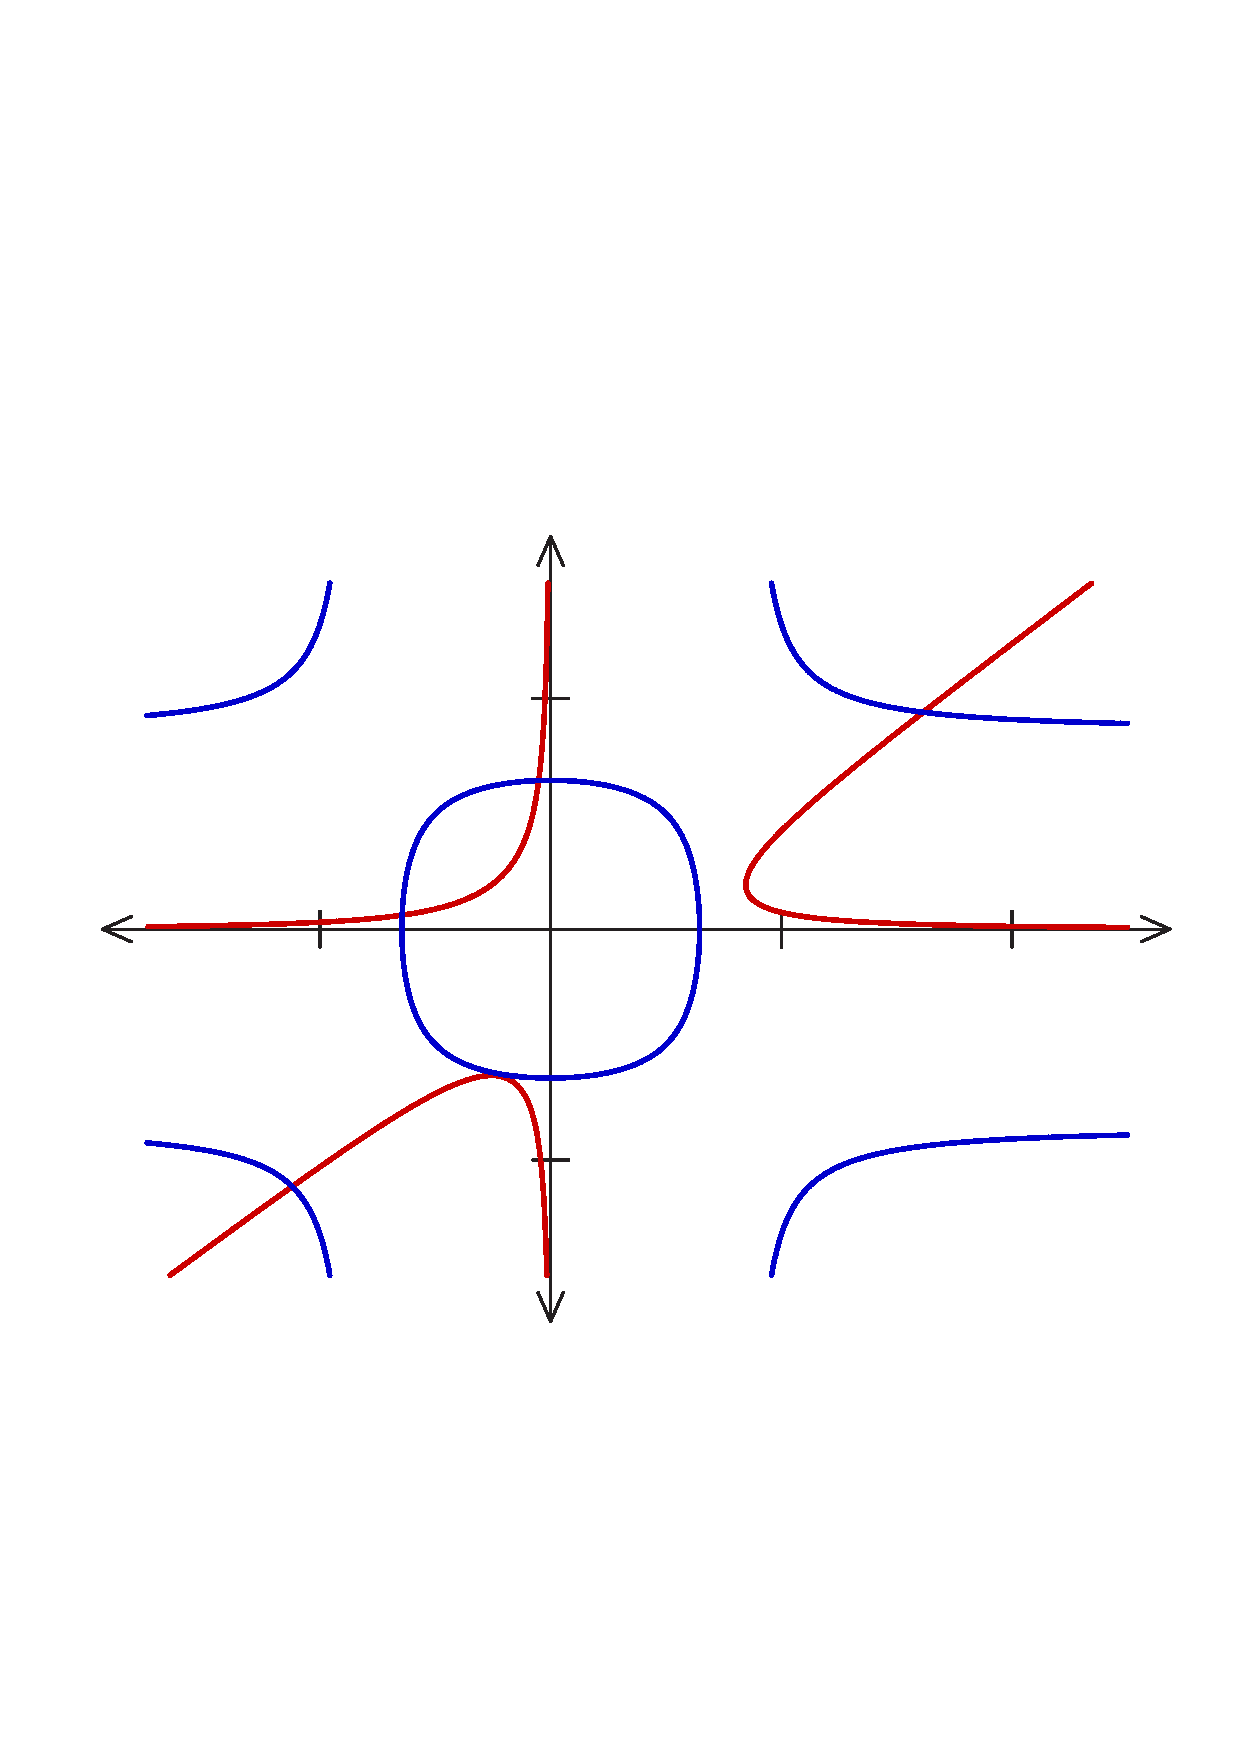
\includegraphics[height=120pt]{pictures/TwoCurves}}
\]
%Trace form is Thm 4.72 in BPR
%
%Sylvester's theorem  is Thm. 2.55 in BPR
%




\bibliographystyle{abbrv}
%\bibliographystyle{amsplain}
\bibliography{jsag}

\end{document}
